\chapter*{Week 12: Objects Continued}
\addcontentsline{toc}{chapter}{Week 12: Objects Continued}
\setcounter{chapter}{13}
\setcounter{section}{0}

\begin{abstract}
This week you will:
\begin{enumerate}
    \item Continue practicing with Objects

\end{enumerate}
    
\end{abstract}

\section{PreQuiz}
\begin{problem}
True or False: In C++, you must explicitly define a constructor for a struct, or it will not compile.
\end{problem}

\begin{problem}
True or False: In C++, you must explicitly define a constructor for a class, or it will not compile.
\end{problem}

\begin{problem}
True or False: Within C++, we separate our code to capture the definition in header files and the implementation within source files.
\end{problem}

\begin{problem}
Short Answer: What is the difference between Data Members and Member Functions?
\end{problem}

\begin{problem}
Short Answer: Explain why a struct might be preferred over a class when defining a simple data container in C++.
\end{problem}

\begin{problem}
Code Analysis: Identify the issue(s) in the following code snippet.
\begin{minted}{c++}
struct City {
    string name;
    int population;

    City(string cityName) {
        name = cityName;
    }
};

int main() {
    City c1("Paris");
    cout << c1.population;
    return 0;
}
\end{minted}
\end{problem}

\begin{problem}
Fill in the blanks in the code below to complete a class that models a guitar with its brand and the number of strings:

\begin{minted}{c++}
#include <iostream>
using namespace std;

class ____ {
public:
    ____ (string b, int s) {
        brand = b;
        strings = s;
    }

    void ____ (int s) {
        ____ = s;
    }

    int ____() const {
        return ____;
    }

    string ____() const {
        return ____;
    }

private:
    string ____;
    int ____;
};

int main() {
    ____ guitar("Fender", 6);
    cout << "Brand: " << guitar.____() << endl;
    cout << "Strings: " << guitar.____() << endl;
    return 0;
}
\end{minted}

\end{problem}



\section{Recitation}
%Player Class from the final project, done in separate stations.

This week you will create a class to represent a player in the game you are creating for your final project. Your final project will be based on the Game of Life, redesigned to take place in the world of the Lion King. Players will journey across the African Savannah, each as a young lion eager to prove they’re ready to step up as the next 'Pride Leader' after Simba’s retirement. Along the way, they’ll make strategic decisions, face unexpected challenges, and collect Pride Points as they grow and refine their Leadership Traits—Stamina, Strength, and Wisdom. For your player objects you will need to keep track of a few details including the name of the player, their in-game age, and then a few statistics to keep track of in-game points: stamina, wisdom, strength, and total points. All of these numerical values can be integers.

\subsection{Header File}

You will need to start by composing a header file where you write your class interface. We suggest having these data members:

\begin{minted}{c++}
string _name;
int _strength, _stamina, _wisdom, _pride_points, _age;
\end{minted}

You will then need to add member functions to your public interface. We will be focusing on four key types of functions:

\begin{enumerate}
    \item Constructors
    \item Getters
    \item Setters
    \item Other member functions
\end{enumerate}

You can start with functions you think would be valuable in all four categories. We will also encourage particular functions as the activity continues. 

You should create a source file and a driver file at this point. For each of the following sections you will go to one location around the room to work on that component. You may work on the following sections in any order. 

In each section, we will outline minimum functions. However, you are allowed to be flexible in how you choose to design this class -- if there is something you believe would be better for usage in your final project, talk to your LAs or TA about your alternative functions.

\subsection{Constructors}

You will need to create a default constructor and at least one parameterized constructor. You should construct the Players so that they start in the accepted range of starting values. All new Player objects should be restricted to these values:

\begin{itemize}
\item Age: 1-20 years old
\item Stamina: 100 - 1000 Points
\item Strength: 100 - 1000 Points
\item Wisdom: 100 - 1000 Points
\end{itemize}

As the Players progress through the game their stats may deviate from these values, but they should start in this range.

The two suggested constructors are as follows:

\textbf{Constructor Functions (public)}

\renewcommand{\arraystretch}{1.5} 
\begin{longtable}{|p{2.0in}|p{4.0in}|}
\hline
\textbf{Function} & \textbf{Description} \\ \hline

\texttt{Default constructor} & Creates a new instance of \mintinline{c++}{Player} by setting \mintinline{c++}{_name} to an empty string, and all numerical values to their minimum accepted value. \\ \hline

\begin{minted}[breaklines=true]{c++}
Player(string name, int strength, int stamina, int wisdom);
\end{minted} 
& Creates a new instance of \mintinline{c++}{Player} with \mintinline{c++}{_name}, \mintinline{c++}{_strength}, \mintinline{c++}{_stamina} and \mintinline{c++}{_wisdom} coming from the parameters. If the parameters are outside of the accepted range of values, use the minimum accepted value instead. \mintinline{c++}{_pride_points} should default to 0, and \mintinline{c++}{_age} should default to 1. \\ \hline

\end{longtable}

\subsection{Getters}

You should create getters for all of your data members. We suggest these:

\textbf{Getter Functions (public)}

\renewcommand{\arraystretch}{1.5} 
\begin{longtable}{|p{2.0in}|p{4.0in}|}
\hline
\textbf{Function} & \textbf{Description} \\ \hline

\mintinline{c++}{string getName();} & return the \mintinline{c++}{_name} data member.\\ \hline
\mintinline{c++}{int getStrength();} & return the \mintinline{c++}{_strength} data member.\\ \hline
\mintinline{c++}{int getStamina();} & return the \mintinline{c++}{_stamina} data member. \\ \hline
\mintinline{c++}{int getWisdom();} & return the \mintinline{c++}{_wisdom} data member.\\ \hline
\mintinline{c++}{int getPridePoints();} & return the \mintinline{c++}{_pride_points} data member.\\ \hline
\mintinline{c++}{int getAge();} & return the \mintinline{c++}{_age} data member.\\ \hline

\end{longtable}

\subsection{Setters}

You should create setters for all of your data members. For each of these functions you should determine whether you would like to return confirmation if a value is updated (create a boolean function) or not (create a void function). 

You might find it more helpful to make these addition functions instead, where we add the parameter to the data member instead of replacing the data member. This may make it easier for you to update values as the game progresses. For example, if you wanted to increase the stamina value by 50, you could either use normal getters and setters like so:

\begin{minted}[breaklines = true]{c++}
    player1.setStamina(player1.getStamina()+50); //get the current stamina value, add 50 to it. Then set the stamina to that value.
\end{minted}

Or you could use an add to stamina function:

\begin{minted}[breaklines = true]{c++}
    player1.addStamina(50); //adds 50 stamina to whatever the current stamina value is.
\end{minted}

You may even want to create both versions. This is entirely up to you. We will suggest the void versions of classic setters below, but feel free to make changes as you see fit:

\textbf{Setter Functions (public)}

\renewcommand{\arraystretch}{1.5} 
\begin{longtable}{|p{3.0in}|p{3.0in}|}
\hline
\textbf{Function} & \textbf{Description} \\ \hline
\mintinline{c++}{void setName(string name);} & update the stored name for your Player \\ \hline
\mintinline{c++}{void setStrength(int strength);} & update the stored strength \\ \hline
\mintinline{c++}{void setStamina(int stamina);} & update the stored stamina \\ \hline
\mintinline{c++}{void setWisdom(int wisdom);} & update the stored wisdom\\ \hline
\mintinline{c++}{void setPridePoints(int pride_points);} & update the stored pride points \\ \hline
\mintinline{c++}{void setAge(int age);} & update the stored age \\ \hline
\end{longtable}

\subsection{Other Member Functions}

You should determine what other member functions might be helpful that go beyond simply getting and setting data values. Three functions are strongly encouraged:

\textbf{Other Functions (public)}

\renewcommand{\arraystretch}{1.5} 
\begin{longtable}{|p{2.0in}|p{4.0in}|}
\hline
\textbf{Function} & \textbf{Description} \\ \hline
\begin{minted}[breaklines=true]{c++}
void trainCub(int strength, int stamina, int wisdom);
\end{minted} 
& This function can be called with a player chooses to train their cub at the start of the game instead of going straight to the pride lands. This should increase the cub's strength, stamina, and wisdom by the parameters given. It should also decrease the pride points by -5,000. \\ \hline
\mintinline{c++}{void toPrideLands();} & This function can be called when a player chooses to go straight to the pride lands at the start of the game and skip training. This should give the player an immediate boost of +5,000 Pride Points, but come at the cost of reduced Strength (-2,000), Wisdom (-2,000), and Stamina (-1,000). \\ \hline
\mintinline{c++}{void printStats();} & This function should print all of the data members in an organized stats message. You can design this message however you like. Here are a few examples:

\begin{example}
Simple stats:

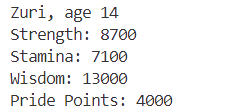
\includegraphics[]{images/project2/PrintStats1.png}
\end{example}

\begin{example}
Stats with a border:

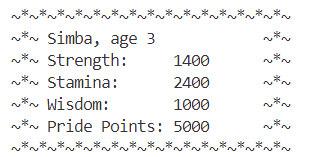
\includegraphics[]{images/project2/PrintStats2.png}
\end{example}

\begin{example}
Stats with ASCII art:

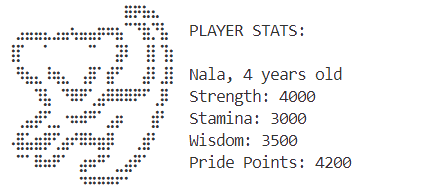
\includegraphics[]{images/project2/PrintStats3.png}
\end{example}

\\ \hline
\end{longtable}

%No homework this week